%\documentclass[12pt,twoside,parskip,solutions]{handout}
\documentclass[12pt,twoside,parskip]{handout}

% Normally the information below would be placed, as appropriate, in files named CourseInfo.tex and UnitInfo.tex, but they have been included in this document in the interest of having only a single file.
% In this case, I would have input those files here:
%\input{../CourseInfo}
%\input{UnitInfo}

% In CourseInfo.tex:
\course{Algebra 1B}
\schoolyear{2019--20}
\block{4}

\renewcommand{\TitleFont}{\huge}
\renewcommand{\FirstPageHeader}{\PSLheader*%
	{\SquircleInnerLine{.75in}{}{}}%
	{b}{\singlespacing\SchoolYear\\{\CourseNameFont\CourseName}\\{\SchoolNameFont\SchoolName}}%
	{b}{{\TitleFont\FancyTitle}\\[\fill]\NameLine}}

% In UnitInfo.tex:
\unit{Quadratics}
\unitnumber{5}

% Ok, back to the handout at hand:
\sheetnumber{6}
\title{Advanced Factoring}

\begin{document}
Last handout, we did a lot of factoring, which we paired with the zero-product rule to solve quadratic equations.
Pretty sweet!

But now that I look back at it, almost all of the quadratics you worked with had a leading coefficient of $a=1$.
Well, that's about to change!
Our factored quadratics are going to need a few more moving pieces, so I like to keep everything organized with a handy grid.

\begin{example*}
	Let's say I want to expand $(2x+5)(-3x+1)$.
	I'd put one factor on the top and the other on the side, then fill in the grid\ldots
	\begin{center}
		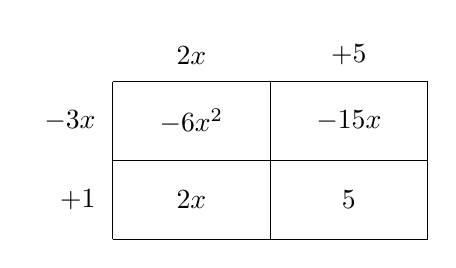
\begin{tikzpicture}[xscale={2}, every node/.append style={inner sep=6pt}]
				\node[anchor=south] at (1,-0.5) {$2x$};
				\node[anchor=south] at (2,-0.5) {$+5$};
			\node[anchor=east] at (0.5,-1) {$-3x$};
			\node[anchor=east] at (0.5,-2) {$+1$};
			
			\node at (1,-1) {$-6x^2$};  \node at (2,-1) {$-15x$};
			\node at (1,-2) {$2x$};     \node at (2,-2) {$5$};
			
			\draw[shift={(0.5,-0.5)}] (0,0) grid (2,-2);
		\end{tikzpicture}
	\end{center}
	\ldots\ and then add it all together: $(2x+5)(-3x+1) = -6x^2 - 15x + 2x + 5 = -6x^2 - 13x + 5$.
	Done!
\end{example*}

\begin{prob}
	\begin{prob}[spaces=.25, columns=2]
		\begin{prob*}
			Expand $(3x+7)(x-2)$

			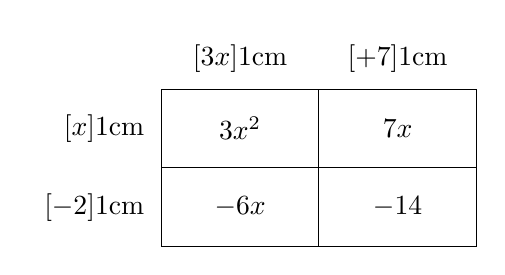
\begin{tikzpicture}[xscale={2}, every node/.append style={inner sep=6pt}]
					\node[anchor=south] at (1,-0.5) {\blank[$3x$]{1cm}};
					\node[anchor=south] at (2,-0.5) {\blank[$+7$]{1cm}};
				\node[anchor=east] at (0.5,-1) {\blank[$x$]{1cm}};
				\node[anchor=east] at (0.5,-2) {\blank[$-2$]{1cm}};
				
				\node at (1,-1) {\ifsoln{$3x^2$}};  \node at (2,-1) {\ifsoln{$7x$}};
				\node at (1,-2) {\ifsoln{$-6x$}};   \node at (2,-2) {\ifsoln{$-14$}};
				
				\draw[shift={(0.5,-0.5)}] (0,0) grid (2,-2);
			\end{tikzpicture}
			\solution
			$3x^2+x-14$
		\end{prob*}
		\begin{prob*}
			Expand $(3x-2)(x+7)$

			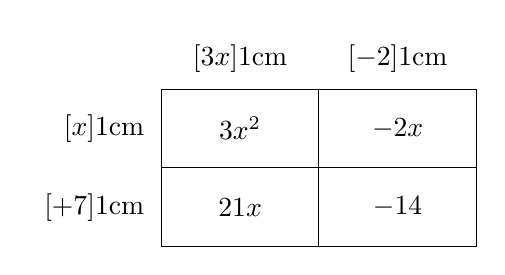
\begin{tikzpicture}[xscale={2}, every node/.append style={inner sep=6pt}]
					\node[anchor=south] at (1,-0.5) {\blank[$3x$]{1cm}};
					\node[anchor=south] at (2,-0.5) {\blank[$-2$]{1cm}};
				\node[anchor=east] at (0.5,-1) {\blank[$x$]{1cm}};
				\node[anchor=east] at (0.5,-2) {\blank[$+7$]{1cm}};
				
				\node at (1,-1) {\ifsoln{$3x^2$}};  \node at (2,-1) {\ifsoln{$-2x$}};
				\node at (1,-2) {\ifsoln{$21x$}};   \node at (2,-2) {\ifsoln{$-14$}};
				
				\draw[shift={(0.5,-0.5)}] (0,0) grid (2,-2);
			\end{tikzpicture}
			\solution
			$3x^2+19x-14$
		\end{prob*}
	\end{prob}
	\begin{prob}[discuss]
		Do you notice anything interesting about the two diagonal pairs of terms in each grid?\\
		(E.g., $-6x^2$ \& $5$\ \ and\ \ $-15x$ \& $2x$ in the example.)
		\solution
		They have the same product! Woah!
	\end{prob}
\end{prob}

\spoilerbreak

\begin{prob}
	Maybe you noticed that both diagonals have the same product.
	Show me why that's the case:
	\begin{center}
		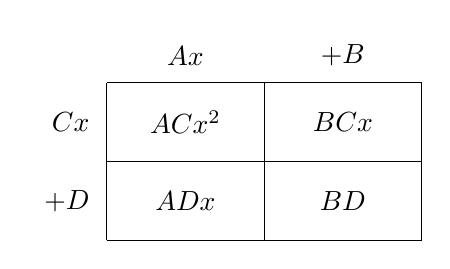
\begin{tikzpicture}[xscale={2}, every node/.append style={inner sep=6pt}]
				\node[anchor=south] at (1,-0.5) {$Ax$};
				\node[anchor=south] at (2,-0.5) {$+B$};
			\node[anchor=east] at (0.5,-1) {$Cx$};
			\node[anchor=east] at (0.5,-2) {$+D$};
			
			\node at (1,-1) {\ifsoln{$ACx^2$}};  \node at (2,-1) {\ifsoln{$BCx$}};
			\node at (1,-2) {\ifsoln{$ADx$}};   \node at (2,-2) {\ifsoln{$BD$}};
			
			\draw[shift={(0.5,-0.5)}] (0,0) grid (2,-2);
		\end{tikzpicture}
	\end{center}
	\solution
	Both diagonals have a product of $ABCDx^2$, and so they are equal.
\end{prob}

\begin{prob}
	Suppose $A$, $B$, $C$, and $D$ are numbers such that 
	\[
		(Az+B)(Cz+D)=12z^2-8z-15.
	\]
	
	\begin{prob}[space=1.5]
		Find $A, B, C$, and $D$.
		\solution
		$A=2$, $B=-3$, $C=6$, and $D=5$
	\end{prob}
	\begin{prob}
		Find all solutions to $12z^2-8z-15=0$.
		\solution
		$z=\frac{3}{2}, \frac{-5}{6}$
	\end{prob}
\end{prob}

\newpage

\begin{prob}[columns=2]
	Factor each of the following.
	
	\begin{prob}
		$6x^2 - 5x + 1$
		\solution
		$(3x - 1)(2x - 1)$
	\end{prob}
	\begin{prob}
		$4x^2 - 2x - 12$
		\solution
		$2(x - 2)(2x + 3)$, or equivalent
	\end{prob}
	\begin{prob}
		$3x^2 + 13x - 10$
		\solution
		$(3x - 2)(x + 5)$
	\end{prob}
	\begin{prob}
		$4x^2 + 7x + 3$
		\solution
		$(x + 1)(4x + 3)$
	\end{prob}
\end{prob}

\newpage

\begin{prob}[exciting]
	Use your factoring skills to find all solutions to the equation $3x^2 + 13x = 10$
	\solution
	Factors as $(3x - 2)(x + 5)=0$, so the solutions are $x=\frac{2}{3}, -5$
\end{prob}

Want an extra challenge?
Try this one!

\begin{prob}[bonus, space=1.5]
	For what values of $k$ can $2x^2+kx+5$ be factored as a product of two linear factors with integer coefficients?
	\solution
	$k=\pm7, \pm 11$
\end{prob}

\spoilerbreak[When you finish, ask me for the next handout!]

\end{document}
